\documentclass[11pt,a4paper]{article}
\usepackage[margin=25mm]{geometry}
\usepackage{graphicx,amsmath,amssymb,siunitx,booktabs,hyperref,placeins}
\usepackage[american]{babel}
\title{Ultrafast Transient-Grating Spectroscopy of GaAs}
\author{Dhruv Pisharody \and Ahmet Kavruk \and Angelo Brade\\Rheinische Friedrich--Wilhelms--Universität Bonn}
\date{}
\begin{document}
\maketitle

\begin{abstract}
Transient-grating spectroscopy probes carrier relaxation and spatial diffusion through the decay of a photoinduced grating. This report analyzes the supplied GaAs autocorrelation, spectrum, pump--probe and transient-grating traces. Complete autocorrelation scans yield selected pulse-duration estimates of \SI{81.7}{fs} before and \SI{79.0}{fs} after the compressor; their small formal fit errors do not include scan-calibration uncertainty. Biexponential fits describe the transient traces over the selected interval, while the slow finite-wave-vector rates give an exploratory ambipolar diffusivity of $(3.71\pm0.70)\times10^{-3}\,\si{\metre\squared\per\second}$. The pump--probe rate is inconsistent with the transient-grating extrapolation, limiting the physical interpretation of that estimate. The data do not directly measure hot-carrier temperature or electron--phonon coupling.
\end{abstract}

\tableofcontents
\clearpage

\section{Introduction}
Ultrafast optical pulses create and probe non-equilibrium carriers in semiconductors. Their temporal relaxation and spatial transport can be studied by measuring the change in reflected or diffracted probe light after excitation. In transient-grating (TG) spectroscopy, two pump beams interfere in the sample and create a periodic carrier-density pattern. Diffusion reduces the grating amplitude, and the decay rate depends on the grating wave number.

This experiment uses GaAs and combines pulse characterization with pump--probe and TG measurements. The analysis follows the four tasks in the course tutorial: determine pulse duration and spectral bandwidth; assess whether the data can determine hot-carrier cooling and electron--phonon coupling; fit transient-reflectivity and TG decay times; and estimate recombination, ambipolar diffusivity and mobility. The report first derives the relevant models, then describes the optical arrangement and supplied data, and finally presents the results in that order. A final discussion compares the results with their assumptions and available literature.

\section{Theoretical background}
\subsection{Transient-grating formation and carrier decay}
An ultrashort pump pulse creates electron--hole pairs in GaAs. Two pump fields with equal intensity $I_0$ and wave vectors $\mathbf{k}_1,\mathbf{k}_2$ produce the intensity pattern
\begin{align}
I(\mathbf{r})&=|E_1+E_2|^2\\
&=|E_1|^2+|E_2|^2+E_1E_2^*+E_1^*E_2\\
&=2I_0\left[1+\cos\left((\mathbf{k}_1-\mathbf{k}_2)\cdot\mathbf{r}+\phi\right)\right].
\end{align}
For an angle $\theta$ between the beams, $q=|\mathbf{k}_1-\mathbf{k}_2|=2k\sin(\theta/2)$ and
\begin{equation}
\Lambda_{\rm TG}=\frac{2\pi}{q}=\frac{\lambda}{2\sin(\theta/2)}.
\end{equation}
The two-beam interference and resulting spatial carrier modulation are illustrated in Fig.~\ref{fig:tutorial-grating}.

\begin{figure}[htbp]
\centering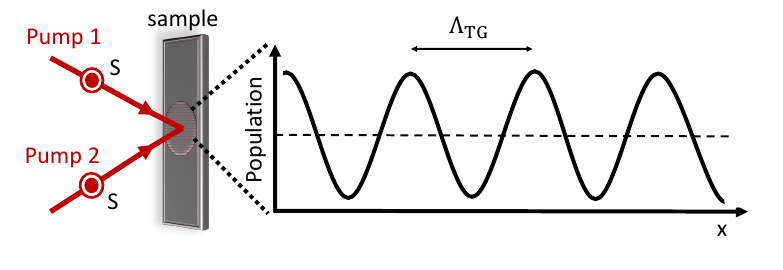
\includegraphics[width=.78\linewidth]{figures/tutorial_grating.png}
\caption{Two crossed pump beams create a sinusoidal excitation pattern in the sample. The grating period $\Lambda_{\rm TG}$ sets the spatial wave number $q=2\pi/\Lambda_{\rm TG}$ used in the diffusion analysis. Reproduced from Fig.~4.5 of the course tutorial.}\label{fig:tutorial-grating}
\end{figure}

Write the carrier density as a uniform part plus its sinusoidal grating component,
\begin{equation}
n(x,t)=N_0(t)+N_q(t)\cos(qx).
\end{equation}
Substitution into the tutorial's one-dimensional diffusion--recombination equation gives
\begin{equation}
\frac{\partial n(x,t)}{\partial t}=D_a\frac{\partial^2 n(x,t)}{\partial x^2}-\frac{n(x,t)}{\tau_{\rm rec}}.
\end{equation}
Using $\partial_t n=\dot N_0+\dot N_q\cos(qx)$ and $\partial_x^2n=-q^2N_q\cos(qx)$, and equating the coefficients of $1$ and $\cos(qx)$, respectively,
\begin{align}
\dot N_0&=-\frac{N_0}{\tau_{\rm rec}}, & \dot N_q&=-\left(D_aq^2+\frac{1}{\tau_{\rm rec}}\right)N_q.\\
\int_{N_0(0)}^{N_0(t)}\frac{dN_0}{N_0}&=-\int_0^t\frac{dt'}{\tau_{\rm rec}}, &
\int_{N_q(0)}^{N_q(t)}\frac{dN_q}{N_q}&=-\int_0^t\left(D_aq^2+\frac{1}{\tau_{\rm rec}}\right)dt'.
\end{align}
Evaluation yields
\begin{align}
N_0(t)&=N_0(0)e^{-t/\tau_{\rm rec}},\\
N_q(t)&=N_q(0)e^{-(D_aq^2+1/\tau_{\rm rec})t}.
\end{align}
For signals proportional to these populations, the $q=0$ transient-reflectivity and finite-$q$ grating traces therefore have the forms
\begin{align}
 S_{\mathrm{pop}}(t)&=A_{\mathrm{pop}}e^{-t/\tau_{\mathrm{rec}}}+C_{\mathrm{pop}},\\
 S_{\mathrm{TG}}(t)&=A_{\mathrm{TG}}e^{-t/\tau_{\mathrm{TG}}}+C_{\mathrm{TG}},\\
 \frac{1}{\tau_{\mathrm{TG}}}&=\frac{1}{\tau_{\mathrm{rec}}}+D_aq^2.
\end{align}
In $1/\tau_{\rm TG}=1/\tau_{\rm rec}+D_aq^2$, the intercept is $1/\tau_{\rm rec}$ and the slope is $D_a$.

The provided measurement instructions request two decay components to represent faster carrier relaxation and slower processes such as grating diffusion. We therefore use the phenomenological extension
\begin{equation}
S(t,q)=C+A_f e^{-t/\tau_f}+A_s e^{-t/\tau_s},\qquad 0<\tau_f<\tau_s.
\end{equation}
The assignments of the two fitted components are interpretations of their timescales. To estimate diffusion, the slow-component rate $1/\tau_s$ is regressed against $q^2$ for the finite-$q$ TG measurements; the single-population diffusion equation above motivates this comparison, but does not by itself derive the biexponential response.

\subsection{Ambipolar transport}
For ambipolar transport, set the excess electron and hole densities equal, $n=h$, and equate their particle fluxes. With the drift--diffusion expressions
\begin{equation}
\mathbf{j}_e=-D_e\nabla n-\mu_en\mathbf{E},\qquad
\mathbf{j}_h=-D_h\nabla n+\mu_hn\mathbf{E},
\end{equation}
the condition $\mathbf{j}_e=\mathbf{j}_h$ gives
\begin{align}
-(D_e-D_h)\nabla n&=(\mu_e+\mu_h)n\mathbf{E},\\
\mathbf{E}&=\frac{D_h-D_e}{\mu_e+\mu_h}\frac{\nabla n}{n},\\
\mathbf{j}_e&=-\left[D_e+\mu_e\frac{D_h-D_e}{\mu_e+\mu_h}\right]\nabla n\\
&=-\frac{D_e\mu_h+D_h\mu_e}{\mu_e+\mu_h}\nabla n.
\end{align}
Comparing with Fick's law $\mathbf{j}=-D_a\nabla n$ identifies
\begin{align}
D_a&=\frac{D_e\mu_h+D_h\mu_e}{\mu_e+\mu_h},\\
D_i&=\frac{k_BT}{e}\mu_i\quad(i=e,h)\\
\Longrightarrow\quad D_a&=\frac{2\mu_e\mu_h}{\mu_e+\mu_h}\frac{k_BT}{e}=\mu_a\frac{k_BT}{e},\\
\mu_a&=\frac{2\mu_e\mu_h}{\mu_e+\mu_h}.
\end{align}
The Einstein step assumes non-degenerate carriers at a common temperature. At high carrier density, many-body and degeneracy effects can change $D_a$ \cite{young}.

\subsection{Pulse duration and spectral bandwidth}
For a Gaussian pulse intensity $I(t)=I_0e^{-t^2/(2\sigma_t^2)}$, the intensity autocorrelation is
\begin{align}
G(\tau)&=\int_{-\infty}^{\infty}I(t)I(t-\tau)\,dt\\
&=I_0^2\int_{-\infty}^{\infty}\exp\!\left[-\frac{t^2+(t-\tau)^2}{2\sigma_t^2}\right]dt\\
&=I_0^2e^{-\tau^2/(4\sigma_t^2)}\int_{-\infty}^{\infty}e^{-(t-\tau/2)^2/\sigma_t^2}\,dt\\
&=I_0^2\sqrt{\pi}\sigma_t e^{-\tau^2/(4\sigma_t^2)}.
\end{align}
Here $t^2+(t-\tau)^2=2(t-\tau/2)^2+\tau^2/2$ and the substitution $u=(t-\tau/2)/\sigma_t$ reduces the integral to $\sigma_t\int_{-\infty}^{\infty}e^{-u^2}du=\sqrt{\pi}\sigma_t$. The intensity half-maximum satisfies $e^{-t^2/(2\sigma_t^2)}=1/2$, so $\Delta t_{\rm pulse}=2\sqrt{2\ln2}\,\sigma_t$. The autocorrelation half-maximum satisfies $e^{-\tau^2/(4\sigma_t^2)}=1/2$, so $\Delta t_{\rm AC}=4\sqrt{\ln2}\,\sigma_t=\sqrt{2}\,\Delta t_{\rm pulse}$.

The Gaussian time--bandwidth product follows by Fourier transforming the field envelope $a(t)=\sqrt{I_0}e^{-t^2/(4\sigma_t^2)}$:
\begin{align}
\widetilde a(\nu)&=\int_{-\infty}^{\infty}a(t)e^{-i2\pi\nu t}\,dt\\
&=\sqrt{I_0}\,e^{-4\pi^2\sigma_t^2\nu^2}
\int_{-\infty}^{\infty}\exp\!\left[-\frac{(t+i4\pi\sigma_t^2\nu)^2}{4\sigma_t^2}\right]dt\\
&=2\sqrt{\pi}\sigma_t\sqrt{I_0}\,e^{-4\pi^2\sigma_t^2\nu^2},\\
|\widetilde a(\nu)|^2&=4\pi\sigma_t^2I_0e^{-8\pi^2\sigma_t^2\nu^2}.
\end{align}
At half maximum, $|\widetilde a(\nu)|^2=|\widetilde a(0)|^2/2$, so
\begin{align}
8\pi^2\sigma_t^2\nu^2&=\ln2,\\
\Delta\nu&=2|\nu|=\frac{\sqrt{\ln2}}{\sqrt{2}\pi\sigma_t}.
\end{align}
Combining this bandwidth with $\Delta t_{\rm pulse}=2\sqrt{2\ln2}\,\sigma_t$ gives
\begin{align}
\Delta t_{\rm pulse}\Delta\nu
&=2\sqrt{2\ln2}\,\sigma_t\frac{\sqrt{\ln2}}{\sqrt{2}\pi\sigma_t}\\
&=\frac{2\ln2}{\pi}\simeq0.441.
\end{align}
From $\nu=c/\lambda$, differentiation gives $d\nu/d\lambda=-c/\lambda^2$; for a narrow spectrum centered at $\lambda_0$, $\Delta\nu\simeq(c/\lambda_0^2)\Delta\lambda$.

The optical pulse duration can be measured with a second-order autocorrelator based on second-harmonic generation (SHG). The measured intensity is a function of the relative delay between two pulse replicas. For a Gaussian pulse, the intensity autocorrelation FWHM is $\sqrt{2}$ times the pulse-intensity FWHM. The transform-limited Gaussian time-bandwidth product is $\Delta t\Delta\nu\simeq0.441$; a larger product can indicate spectral phase/chirp, or measurement and calibration errors. A spectrometer measures wavelength, with $\Delta\nu\simeq c\Delta\lambda/\lambda_0^2$ for a narrow spectrum. This conversion and the time-bandwidth comparison assume that the fitted spectral profile is representative of the pulse spectrum and approximately Gaussian.

\subsection{Derivation of the measured interferometric autocorrelation}
The measured second-order autocorrelation is given in the tutorial by Eq.~(4.2). With $I(t)=|E(t)|^2$, its full expression is
\begin{equation}\tag{4.2}\label{eq:tutorial-iac}
\begin{aligned}
I_{\rm AC}(\tau)={}&\int_{-\infty}^{\infty}\!\left[I^2(t)+I^2(t-\tau)\right]\,\mathrm{d}t\\
&+\int_{-\infty}^{\infty}\!\left[I(t)+I(t-\tau)\right]
\operatorname{Re}\!\left\{E(t)E^*(t-\tau)\right\}\,\mathrm{d}t\\
&+\int_{-\infty}^{\infty}\!\operatorname{Re}\!\left\{E^2(t)E^{*2}(t-\tau)\right\}\,\mathrm{d}t\\
&+\int_{-\infty}^{\infty}\!I(t)I(t-\tau)\,\mathrm{d}t.
\end{aligned}
\end{equation}
For explicit evaluation, take a Gaussian field
\begin{equation}
E(t)=E_0e^{-t^2/(4\sigma^2)}e^{-i\omega_0t},\qquad
I(t)=|E(t)|^2=I_0e^{-t^2/(2\sigma^2)},\qquad I_0=|E_0|^2.
\end{equation}
The Gaussian integral used below is obtained by squaring it and converting to polar coordinates:
\begin{align}
J&=\int_{-\infty}^{\infty}e^{-u^2}\,du,\\
J^2&=\int_{-\infty}^{\infty}\!\int_{-\infty}^{\infty}e^{-(u^2+v^2)}\,du\,dv
=\int_0^{2\pi}\!d\varphi\int_0^\infty e^{-r^2}r\,dr
=2\pi\left[-\frac{e^{-r^2}}{2}\right]_0^\infty=\pi,\\
J&=\sqrt{\pi}.
\end{align}
The four integrals in Eq.~\eqref{eq:tutorial-iac} then evaluate as follows. The first, delay-independent term is
\begin{align}
T_0&=\int_{-\infty}^{\infty}[I^2(t)+I^2(t-\tau)]\,dt\\
&=2I_0^2\int_{-\infty}^{\infty}e^{-t^2/\sigma^2}\,dt
=2I_0^2\sqrt{\pi}\sigma.
\end{align}
For the fundamental-frequency term, first multiply each intensity by the field overlap. The carrier factor is
\begin{equation}
E(t)E^*(t-\tau)=I_0e^{-[t^2+(t-\tau)^2]/(4\sigma^2)}e^{-i\omega_0\tau}.
\end{equation}
The two overlap integrals are equal after completing the square:
\begin{align}
\int_{-\infty}^{\infty} I(t)E(t)E^*(t-\tau)\,dt
&=I_0^2e^{-i\omega_0\tau}\int e^{-[3t^2+(t-\tau)^2]/(4\sigma^2)}\,dt\\
&=I_0^2e^{-i\omega_0\tau}e^{-3\tau^2/(16\sigma^2)}
\int e^{-(t-\tau/4)^2/\sigma^2}\,dt\\
&=I_0^2\sqrt{\pi}\sigma e^{-3\tau^2/(16\sigma^2)}e^{-i\omega_0\tau},\\
\int_{-\infty}^{\infty} I(t-\tau)E(t)E^*(t-\tau)\,dt
&=I_0^2\sqrt{\pi}\sigma e^{-3\tau^2/(16\sigma^2)}e^{-i\omega_0\tau}.
\end{align}
Taking the real part of their sum gives
\begin{equation}
T_1=2I_0^2\sqrt{\pi}\sigma e^{-3\tau^2/(16\sigma^2)}\cos(\omega_0\tau).
\end{equation}
For the second-harmonic field-overlap term,
\begin{align}
E^2(t)E^{*2}(t-\tau)
&=I_0^2e^{-[t^2+(t-\tau)^2]/(2\sigma^2)}e^{-i2\omega_0\tau},\\
T_2&=\operatorname{Re}\int_{-\infty}^{\infty} E^2(t)E^{*2}(t-\tau)\,dt\\
&=I_0^2e^{-\tau^2/(4\sigma^2)}\cos(2\omega_0\tau)
\int e^{-(t-\tau/2)^2/\sigma^2}\,dt\\
&=I_0^2\sqrt{\pi}\sigma e^{-\tau^2/(4\sigma^2)}\cos(2\omega_0\tau).
\end{align}
The final intensity-overlap term has the same Gaussian integral without the cosine:
\begin{align}
T_3&=\int_{-\infty}^{\infty} I(t)I(t-\tau)\,dt\\
&=I_0^2e^{-\tau^2/(4\sigma^2)}\int e^{-(t-\tau/2)^2/\sigma^2}\,dt\\
&=I_0^2\sqrt{\pi}\sigma e^{-\tau^2/(4\sigma^2)}.
\end{align}
Combining these evaluated terms gives the Gaussian-pulse form of Eq.~\eqref{eq:tutorial-iac}:
\begin{equation}
I_{\rm AC}(\tau)=2I_0^2\sqrt{\pi}\sigma+2I_0^2\sqrt{\pi}\sigma e^{-3\tau^2/(16\sigma^2)}\cos(\omega_0\tau)
+I_0^2\sqrt{\pi}\sigma e^{-\tau^2/(4\sigma^2)}[1+\cos(2\omega_0\tau)].
\end{equation}
Thus the integrals explicitly produce fringes at $\omega_0$ and $2\omega_0$. For the measured trace, the fit uses a common Gaussian envelope for the slowly varying terms as a phenomenological approximation to these overlap functions; it fits
\begin{equation}
S(x)=S_0+e^{-(x-x_0)^2/(2\sigma_x^2)}\left[A_0+A_1\cos(2\pi f(x-x_0)+\phi_1)+A_2\cos(4\pi f(x-x_0)+\phi_2)\right].
\end{equation}
In a scan coordinate $x$ with fringe frequency $f$, one optical cycle takes $1/f$ on the recorded axis and $\lambda_0/c$ in delay. Therefore
\begin{align}
\tau-\tau_0&=\frac{\lambda_0}{c}f(x-x_0),\\
\omega_0(\tau-\tau_0)&=\frac{2\pi c}{\lambda_0}\frac{\lambda_0}{c}f(x-x_0)=2\pi f(x-x_0),\\
2\omega_0(\tau-\tau_0)&=4\pi f(x-x_0),
\end{align}
which gives the two cosine arguments in the fit. The fitted Gaussian intensity envelope is
\begin{equation}
I_{\rm env}(x)=A_{\rm env}\exp\!\left[-\frac{(x-x_0)^2}{2\sigma_x^2}\right],
\qquad A_{\rm env}=A_0+|A_1|+|A_2|.
\end{equation}
In the tutorial's field-envelope notation, its square root is
\begin{equation}
E_{\rm env}(x)=\sqrt{I_{\rm env}(x)}=\sqrt{A_{\rm env}}\exp\!\left[-\frac{(x-x_0)^2}{4\sigma_x^2}\right],
\qquad E_{\rm env}^2(x)=I_{\rm env}(x).
\end{equation}
Figure~\ref{fig:autocorrelation} overlays the normalized $E_{\rm env}(x)$ (the square root of the fitted intensity envelope) on the raw signal.
The fit envelope has standard deviation $\sigma_x$ in recorded coordinate. The local scan factor is $d\tau/dx=f\lambda_0/c$, so $\sigma_\tau=(f\lambda_0/c)\sigma_x$. Its FWHM and the pulse FWHM are
\begin{align}
\Delta t_{\rm AC}&=2\sqrt{2\ln2}\,\sigma_\tau
=2\sqrt{2\ln2}\,\sigma_xf\lambda_0/c,\\
\Delta t_{\rm pulse}&=\frac{\Delta t_{\rm AC}}{\sqrt{2}}.
\end{align}

\section{Experimental setup and measurement}
\subsection{Optical arrangement}
The tutorial describes a Kerr-lens mode-locked Ti:sapphire femtosecond laser. Its intensity-dependent refractive index produces self-focusing that favors pulsed operation; a prism compressor compensates dispersion and reduces pulse chirp. For autocorrelation, a Michelson interferometer creates two pulse replicas with adjustable delay and a BBO crystal generates a second-harmonic signal proportional to their temporal overlap. For the sample measurement, the beam is split into pump and probe paths; two pump beams cross on the GaAs sample and make the excitation grating. Two probe beams arranged in BOXCAR geometry provide a diffracted signal and a local oscillator. Their interference gives a heterodyne term proportional to the diffracted field, improving sensitivity over direct intensity detection. The tutorial describes phase modulation of the local oscillator with a rotating coverslip and pump modulation with a chopper; a lock-in amplifier extracts the component at the chopper frequency. The overall optical layout is shown in Fig.~\ref{fig:tutorial-setup}; the individual Michelson autocorrelator and BOXCAR detection principle are shown in Figs.~\ref{fig:tutorial-autocorrelator} and~\ref{fig:tutorial-heterodyne}..

\begin{figure}[htbp]
\centering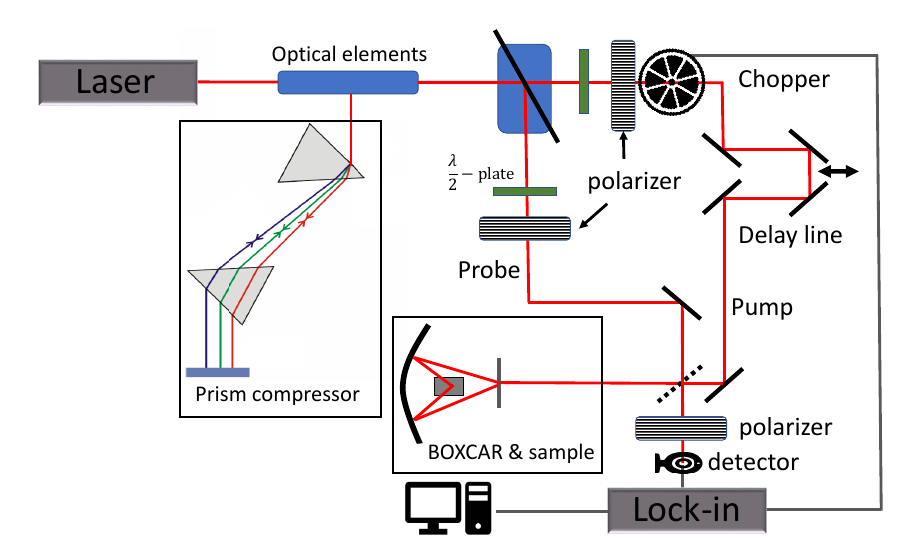
\includegraphics[width=.82\linewidth]{figures/tutorial_setup.png}
\caption{Tutorial schematic of the transient-reflectivity and transient-grating apparatus, including prism compressor, pump and probe paths, delay line, chopper, BOXCAR sample geometry, detector, and lock-in amplifier. Reproduced from Fig.~4.7 of the course tutorial.}\label{fig:tutorial-setup}
\end{figure}
\begin{figure}[htbp]
\centering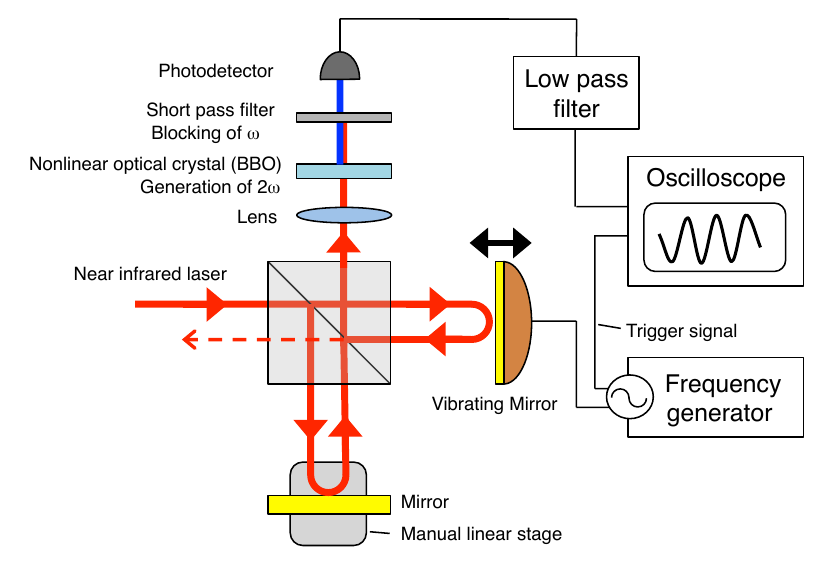
\includegraphics[width=.76\linewidth]{figures/tutorial_autocorrelator.png}
\caption{Michelson autocorrelator schematic: the vibrating mirror varies the relative delay between pulse replicas, and a BBO crystal generates the detected second harmonic. Reproduced from Fig.~4.1 of the course tutorial.}\label{fig:tutorial-autocorrelator}
\end{figure}
\begin{figure}[htbp]
\centering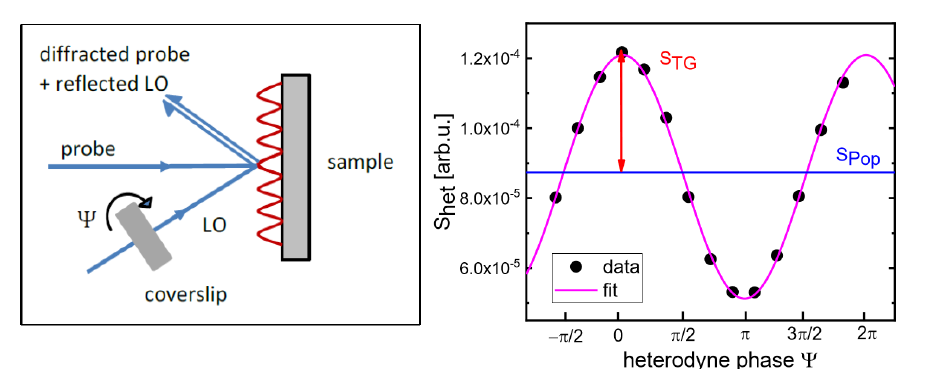
\includegraphics[width=.76\linewidth]{figures/tutorial_heterodyne.png}
\caption{BOXCAR heterodyne detection of the diffracted probe and reflected local oscillator, with the measured signal illustrated as a function of heterodyne phase. Reproduced from Fig.~4.6 of the course tutorial.}\label{fig:tutorial-heterodyne}
\end{figure}

\subsection{Measurement data and calibration}
The supplied data comprise the spectrum file \texttt{spektrum.csv}, three before-compressor traces (\texttt{vor1}--\texttt{vor3}), three after-compressor traces (\texttt{nach1}--\texttt{nach3}), and five transient files: one pump--probe trace and four TG traces. Each transient file contains delay in its first column and repeated scans in the remaining columns. The measurement instructions specify delay in picoseconds and state that the actual sample grating period is one quarter of the phase-mask period encoded in each TG filename; we therefore use $\Lambda_{\rm sample}=\Lambda_{\rm mask}/4$ and $q=2\pi/\Lambda_{\rm sample}$. The exact incidence angles and an independent grating-period calibration were not supplied.

The \texttt{vor2} trace is visibly truncated compared with the other before-compressor scans and has a sampling interval differing by a factor of five. It is therefore not treated as a complete pulse-width candidate. The complete candidates are ranked by normalized fit residual, and the lowest-residual trace in each compressor group is used for the reported pulse duration. The before/after files are shown together in Fig.~\ref{fig:vor-nach}; their different scan extents are apparent there.

\subsection{Data screening and fit procedure}
The analysis was performed with the Python scripts in \texttt{analysis/}. For each TG dataset with at least eight repeats, the scan-level deviation score is the root-mean-square of each scan's difference from the pointwise median, standardized by the larger of the pointwise robust scale $1.4826\,\mathrm{MAD}$ and its lower-quartile floor. Scores are converted to modified scores using $z_j=0.6745(s_j-\mathrm{median}(s))/\mathrm{MAD}(s)$; scans above 3.5 are flagged. The flagged traces are inspected against the retained-scan distribution before exclusion. The quality-screen plots and the direct scan comparison are included with the transient-decay results in Figs.~\ref{fig:outlier-diagnostics} and \ref{fig:excluded-scan-comparison}.

The retained scans are averaged pointwise, with standard errors across repeats. The mean traces are fitted for $t\geq\SI{0.5}{ps}$ to the ordered biexponential model introduced in Sec.~2.1. A 300-replicate bootstrap resamples complete retained scans within each dataset, repeats the averaging and fitting, and propagates slow rates through the finite-$q$ regression. The resulting intervals quantify repeat-scan variability conditional on the selected traces and model. They do not include calibration or model uncertainty.

Several experimental conditions needed for full reproducibility were not recorded in the supplied files: sample temperature, pump and probe fluence, spot size, sample thickness and orientation, incidence angles, and detector/lock-in settings. These missing quantities also limit the comparison with literature measurements.

\section{Results}
\subsection{Part I: Pulse duration and spectral bandwidth}
Pulse duration is obtained by converting the fitted width on the recorded scan coordinate to delay using the local fringe frequency. This conversion assumes a locally constant delay-scan speed. The selected fitted traces are shown in Fig.~\ref{fig:autocorrelation}. We exclude \texttt{vor2}: its recorded scan ends at \SI{2.8}{ms}, compared with \SI{14}{ms} for \texttt{vor1} and \texttt{vor3}, leaving the outer autocorrelation wings incompletely recorded (Fig.~\ref{fig:vor-nach}). Its sampling interval also differs by a factor of five, so its scan calibration is not directly comparable. Including it would bias the before-compressor pulse-width estimate.

\begin{figure}[htbp]
\centering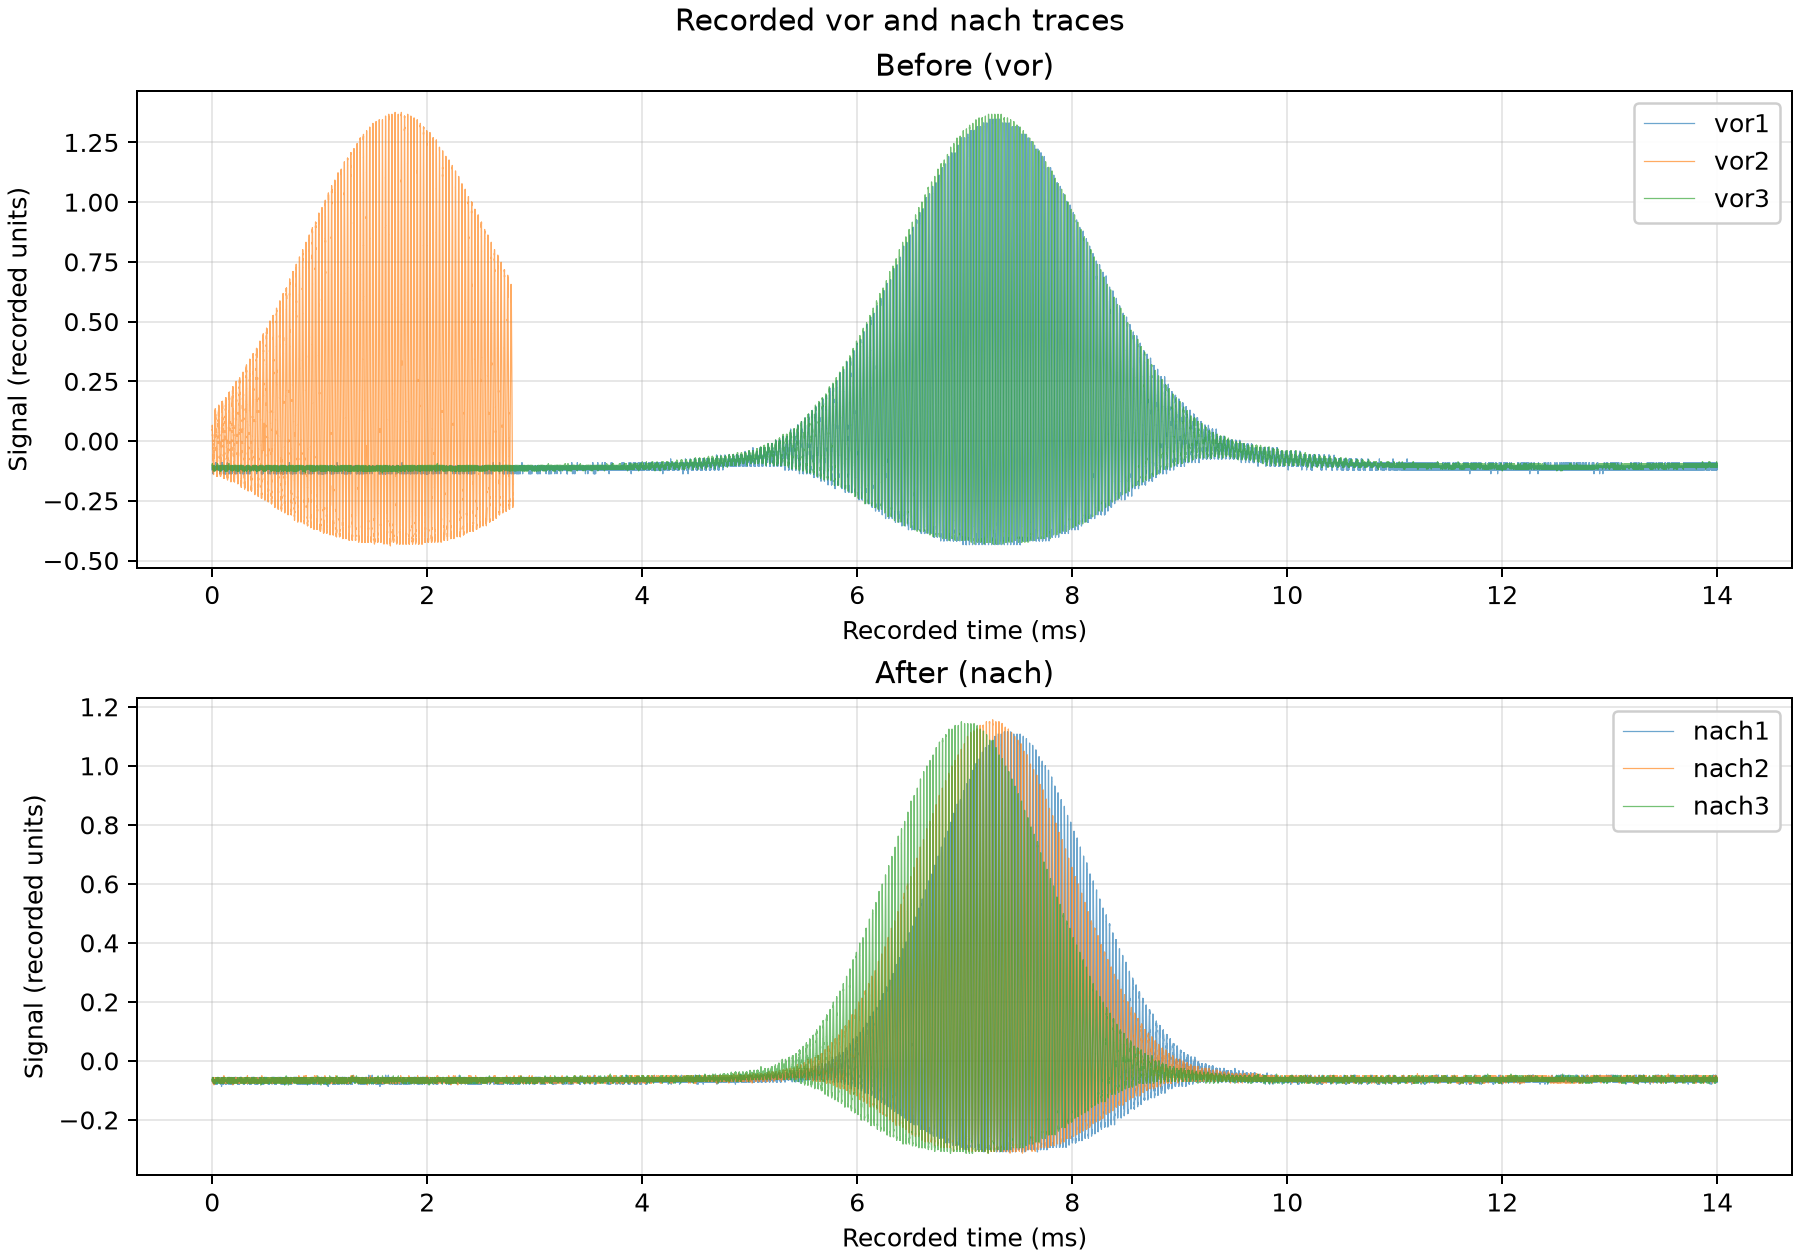
\includegraphics[width=.95\linewidth]{../plots/vor_nach.png}
\caption{Recorded auxiliary traces grouped as before (vor) and after (nach). The horizontal axis uses recorded time converted to milliseconds.}\label{fig:vor-nach}
\end{figure}


The measured spectrum and Gaussian fit are shown in Fig.~\ref{fig:spectrum}. The spectrum file spans approximately \SI{345}{nm} to \SI{1041}{nm}. We fitted all recorded points with
\begin{equation}
S(\lambda)=B+A\exp\!\left[-\frac{(\lambda-\lambda_0)^2}{2\sigma_\lambda^2}\right].
\end{equation}
The peak above baseline is $A$ and the fitted peak level is $B+A$. At half peak height above baseline, $S-B=A/2$, so
\begin{align}
e^{-(\lambda-\lambda_0)^2/(2\sigma_\lambda^2)}&=\frac12,\\
|\lambda-\lambda_0|&=\sqrt{2\ln2}\,|\sigma_\lambda|,\\
\Delta\lambda_{\rm FWHM}&=2\sqrt{2\ln2}\,|\sigma_\lambda|.
\end{align}
The fit gives a centre of \SI{788.66}{nm}, peak intensity of \SI{13302}{a.u.}, median measured intensity of \SI{2501}{a.u.}, and fitted half-maximum level of \SI{7902}{a.u.}; $\Delta\lambda_{\rm FWHM}\approx\SI{10.92}{nm}$. Applying $\Delta\nu\simeq c\Delta\lambda/\lambda_0^2$ gives $\Delta\nu\approx\SI{5.26}{THz}$. The Gaussian time-bandwidth result derived above gives $\Delta t_{\rm TL}=0.441/\Delta\nu\approx\SI{83.8}{fs}$. The median is calculated from all measured spectrum points; it is plotted as a descriptive reference and is not the fitted background $B$.

\begin{figure}[htbp]
\centering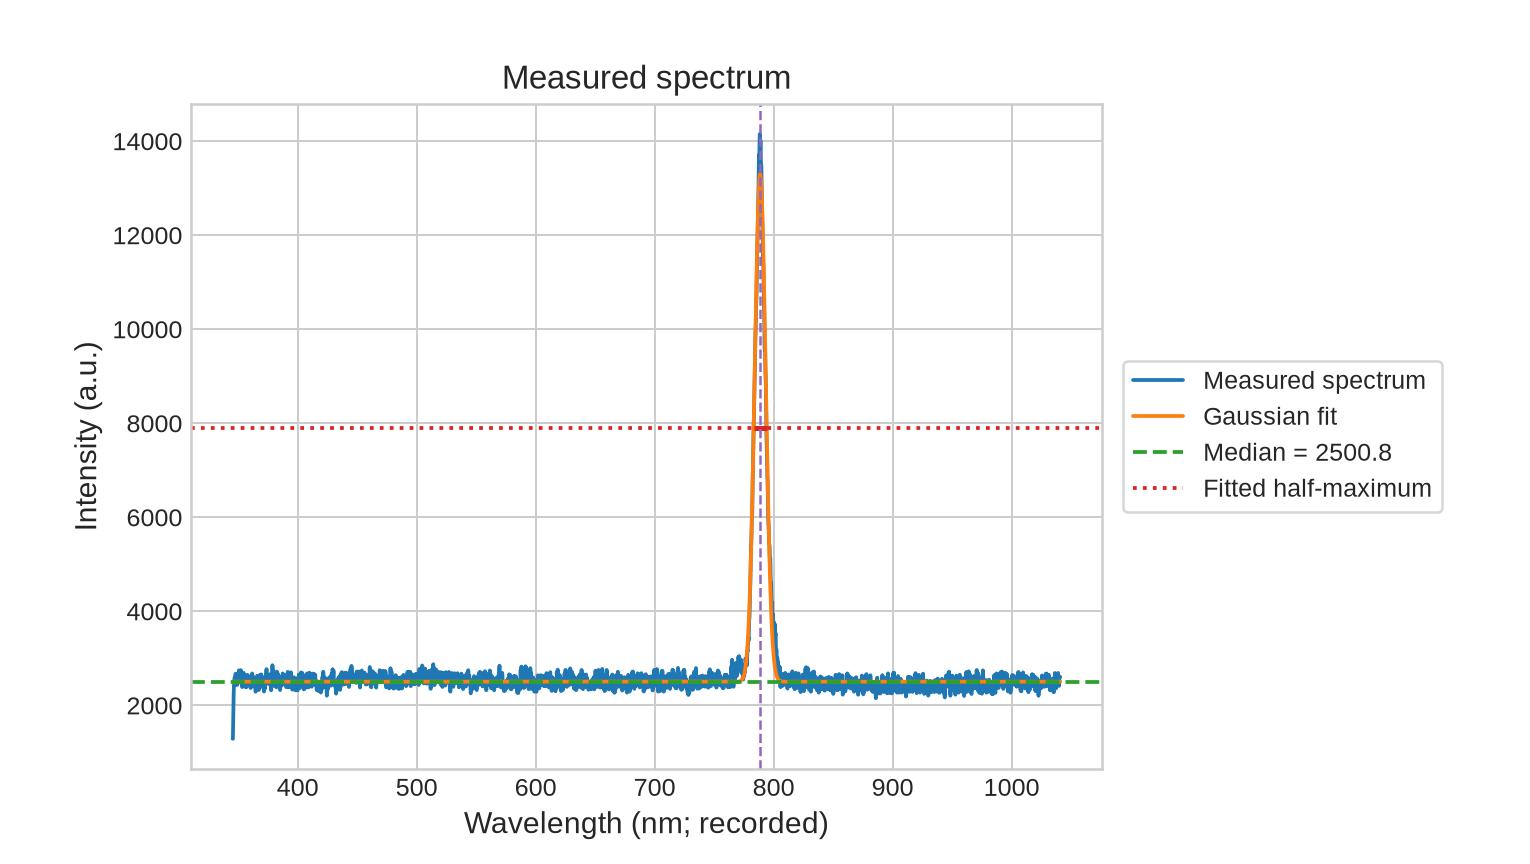
\includegraphics[width=.98\linewidth]{../plots/spectrum.png}
\caption{Measured spectrum, Gaussian fit, median level, and fitted half-maximum bandwidth.}\label{fig:spectrum}
\end{figure}


The normalized fit residuals for the complete autocorrelation candidates are 0.1222 (\texttt{vor1}), 0.1214 (\texttt{vor3}), 0.0922 (\texttt{nach1}), 0.0914 (\texttt{nach2}), and 0.0909 (\texttt{nach3}). Thus \texttt{vor3} and \texttt{nach3} are selected as the cleanest traces under this criterion. Their fitted pulse durations are \SI{81.7}{fs} and \SI{79.0}{fs}, respectively. These are individual selected-trace estimates, not averages over repeats; the corresponding time-bandwidth products are about 0.43 and 0.42. Systematic uncertainty from scan nonlinearity, model assumptions, and instrument response remains unquantified. The reported spectral bandwidth uncertainty ($\pm\SI{0.03}{nm}$) and autocorrelation fit uncertainties ($\pm\SI{0.50}{fs}$ before and $\pm\SI{0.36}{fs}$ after) are formal nonlinear-fit covariance errors only; they exclude calibration, model, and candidate-selection uncertainty. The inferred durations are slightly below the Gaussian transform limit, so these small formal errors should not be read as total experimental uncertainties.

\begin{figure}[htbp]
\centering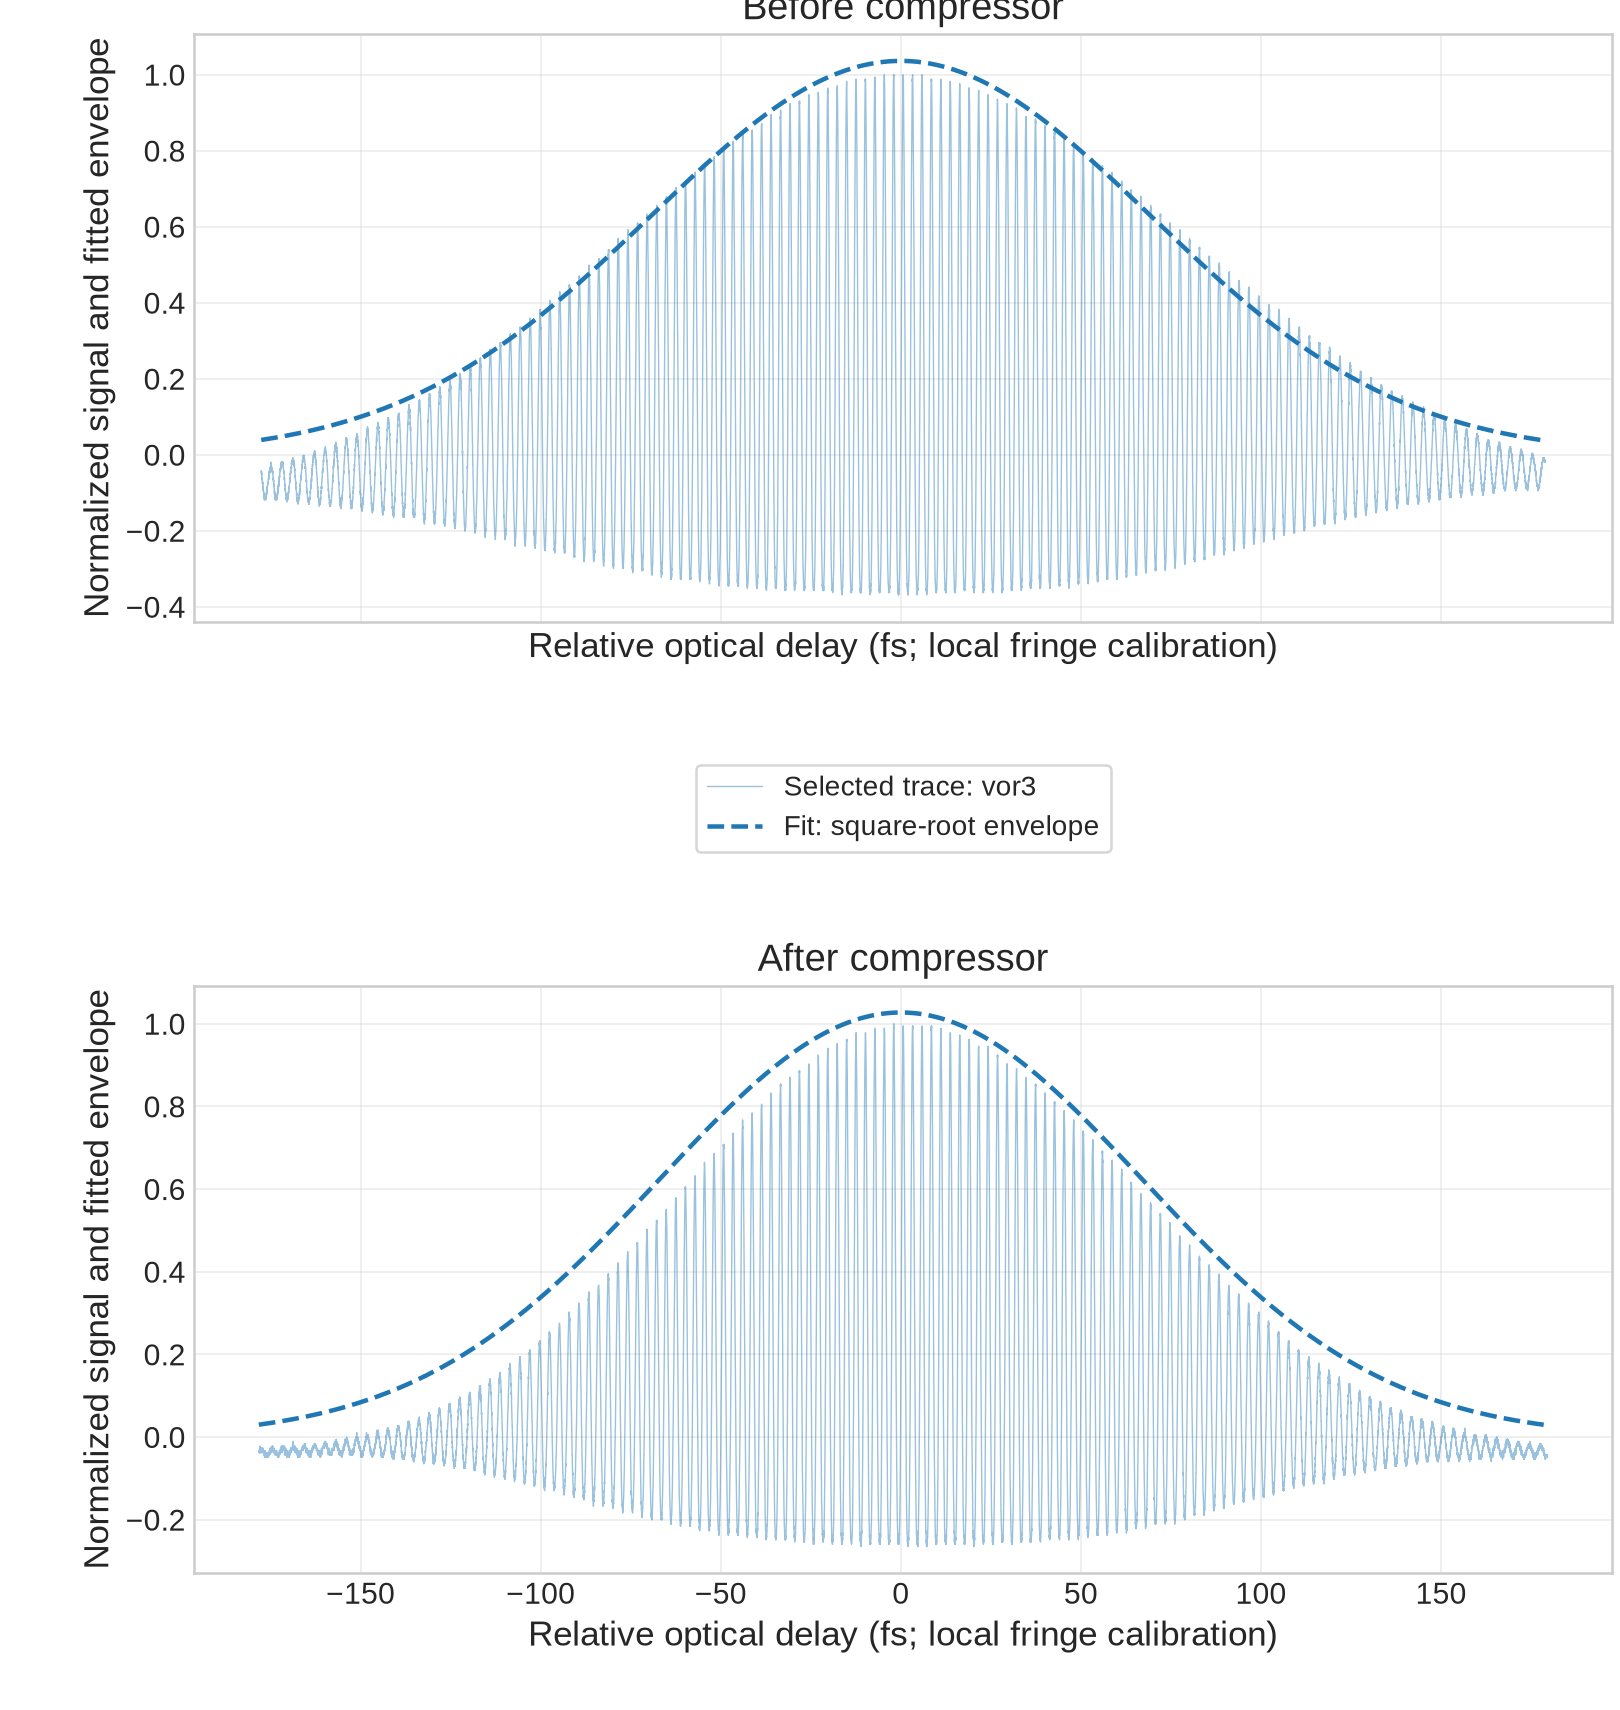
\includegraphics[width=\linewidth]{../plots/autocorrelation_pulsewidth.png}
\caption{Selected cleanest complete before and after autocorrelation traces, \texttt{vor3} and \texttt{nach3}, with fitted square-root Gaussian envelopes. Candidate quality is ranked by normalized fit residual; the truncated \texttt{vor2} scan is excluded.}\label{fig:autocorrelation}
\end{figure}

\FloatBarrier

\subsection{Part II: Hot-carrier cooling and electron--phonon coupling}
The tutorial asks for a hot-carrier cooling time and an average electron--phonon coupling coefficient. These data do not support either quantity as a physical measurement: the reflectivity traces record an optical response, not the carrier temperature or energy distribution, and the biexponential fit is phenomenological. In addition, the fitted interval starts at \SI{0.5}{ps}, so it cannot resolve the subpicosecond thermalization and scattering dynamics. We therefore do not identify $\tau_f$ with a cooling constant or calculate an electron--phonon coupling coefficient from it. For context, GaAs thermalization has been reported on a roughly \SI{200}{fs} scale, and average electron--LO-phonon scattering around \SI{165}{fs} for injected densities below $10^{17}\,\mathrm{cm}^{-3}$; these are microscopic times and are not directly comparable to our fitted reflectivity lifetimes \cite{hunsche,kash}. A defensible cooling constant and coupling estimate would require a calibrated carrier-temperature or energy-versus-delay measurement and the relevant excitation conditions.

\subsection{Part III: Transient-reflectivity and transient-grating decay times}\label{sec:decay-results}
The scan screen flags two period-8 repeats for inspection, as shown in Fig.~\ref{fig:outlier-diagnostics}; their direct comparison with the retained population is in Fig.~\ref{fig:excluded-scan-comparison}. The retained-scan means and biexponential fits are shown in Fig.~\ref{fig:gaas-decay}; Fig.~\ref{fig:fit-residuals} shows residuals normalized by the fitted-window signal range. The normalized residual RMS is 1.26\% for pump--probe and 0.71--0.81\% for TG. The residuals show that the biexponential describes the averaged traces over the fitted interval, but do not establish a unique microscopic assignment.

\begin{figure}[htbp]
\centering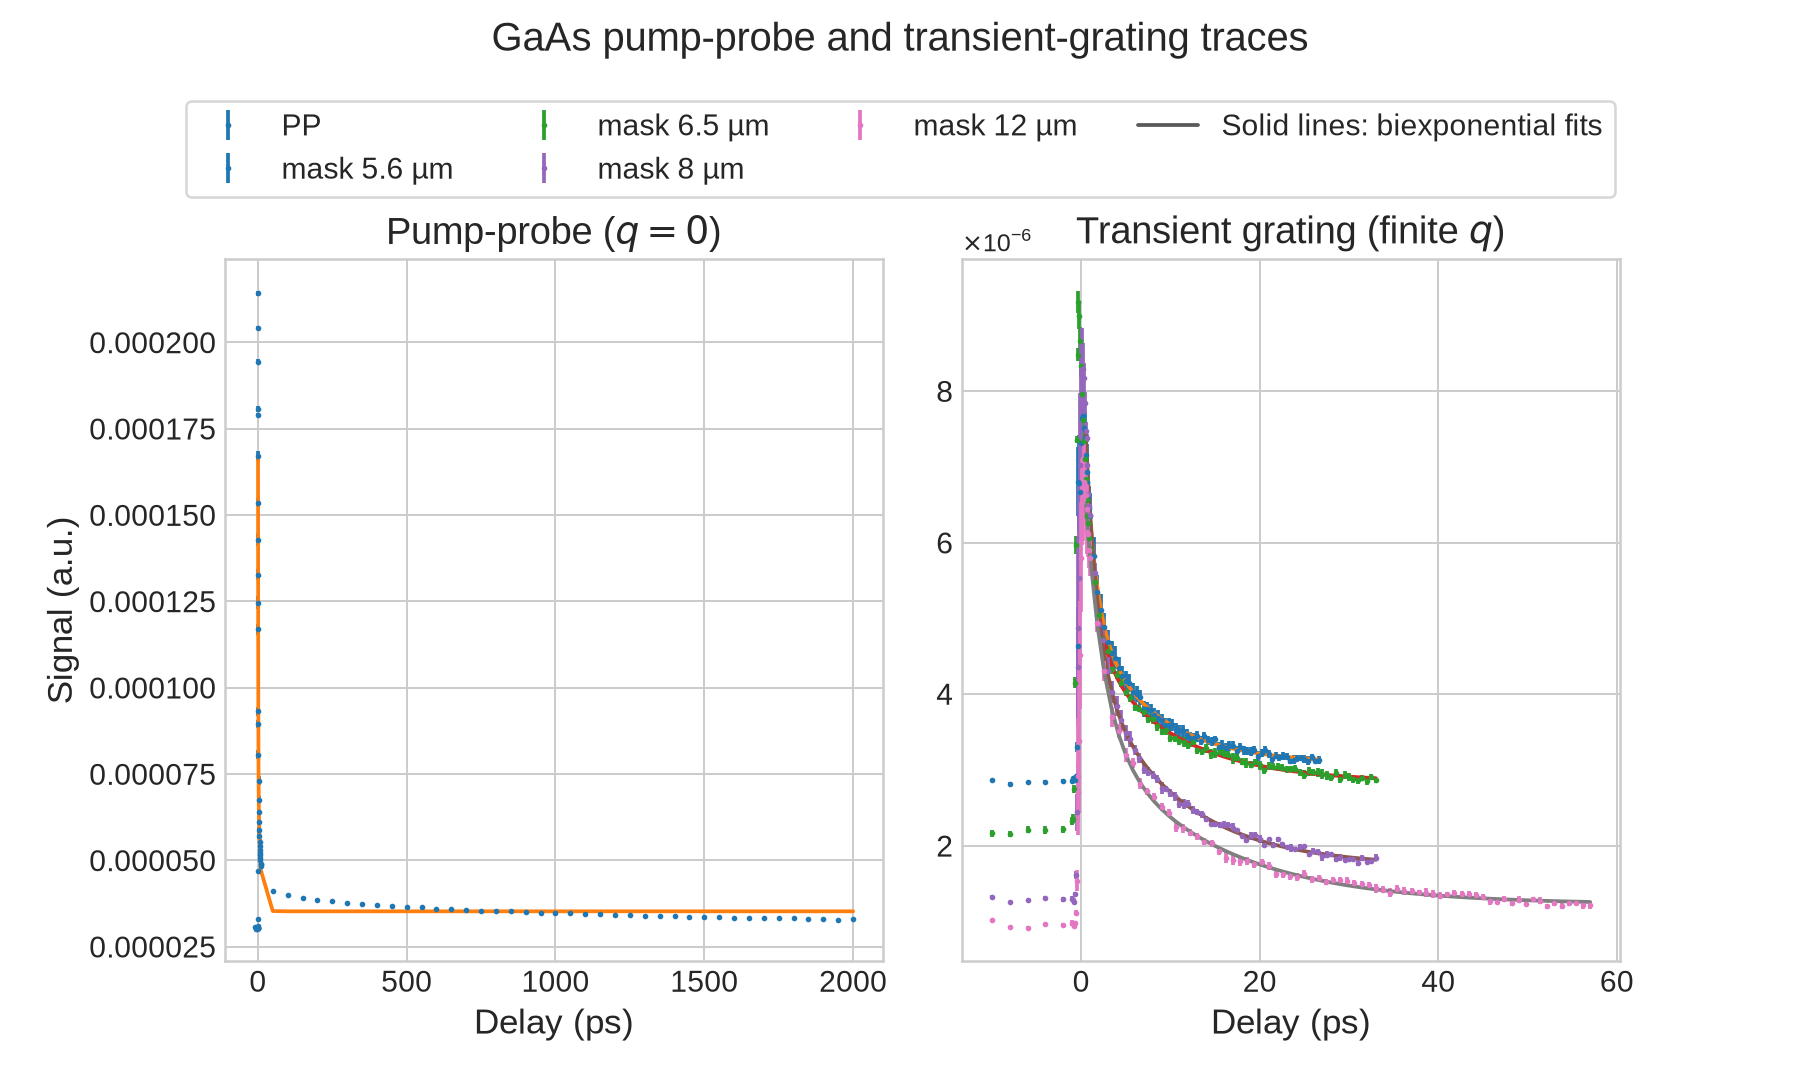
\includegraphics[width=.98\linewidth]{../plots/gaas_decay.png}
\caption{Mean delay traces over retained scans and biexponential fits, with delay in ps. Error bars show the standard error across retained scans.}\label{fig:gaas-decay}
\end{figure}
\begin{figure}[htbp]
\centering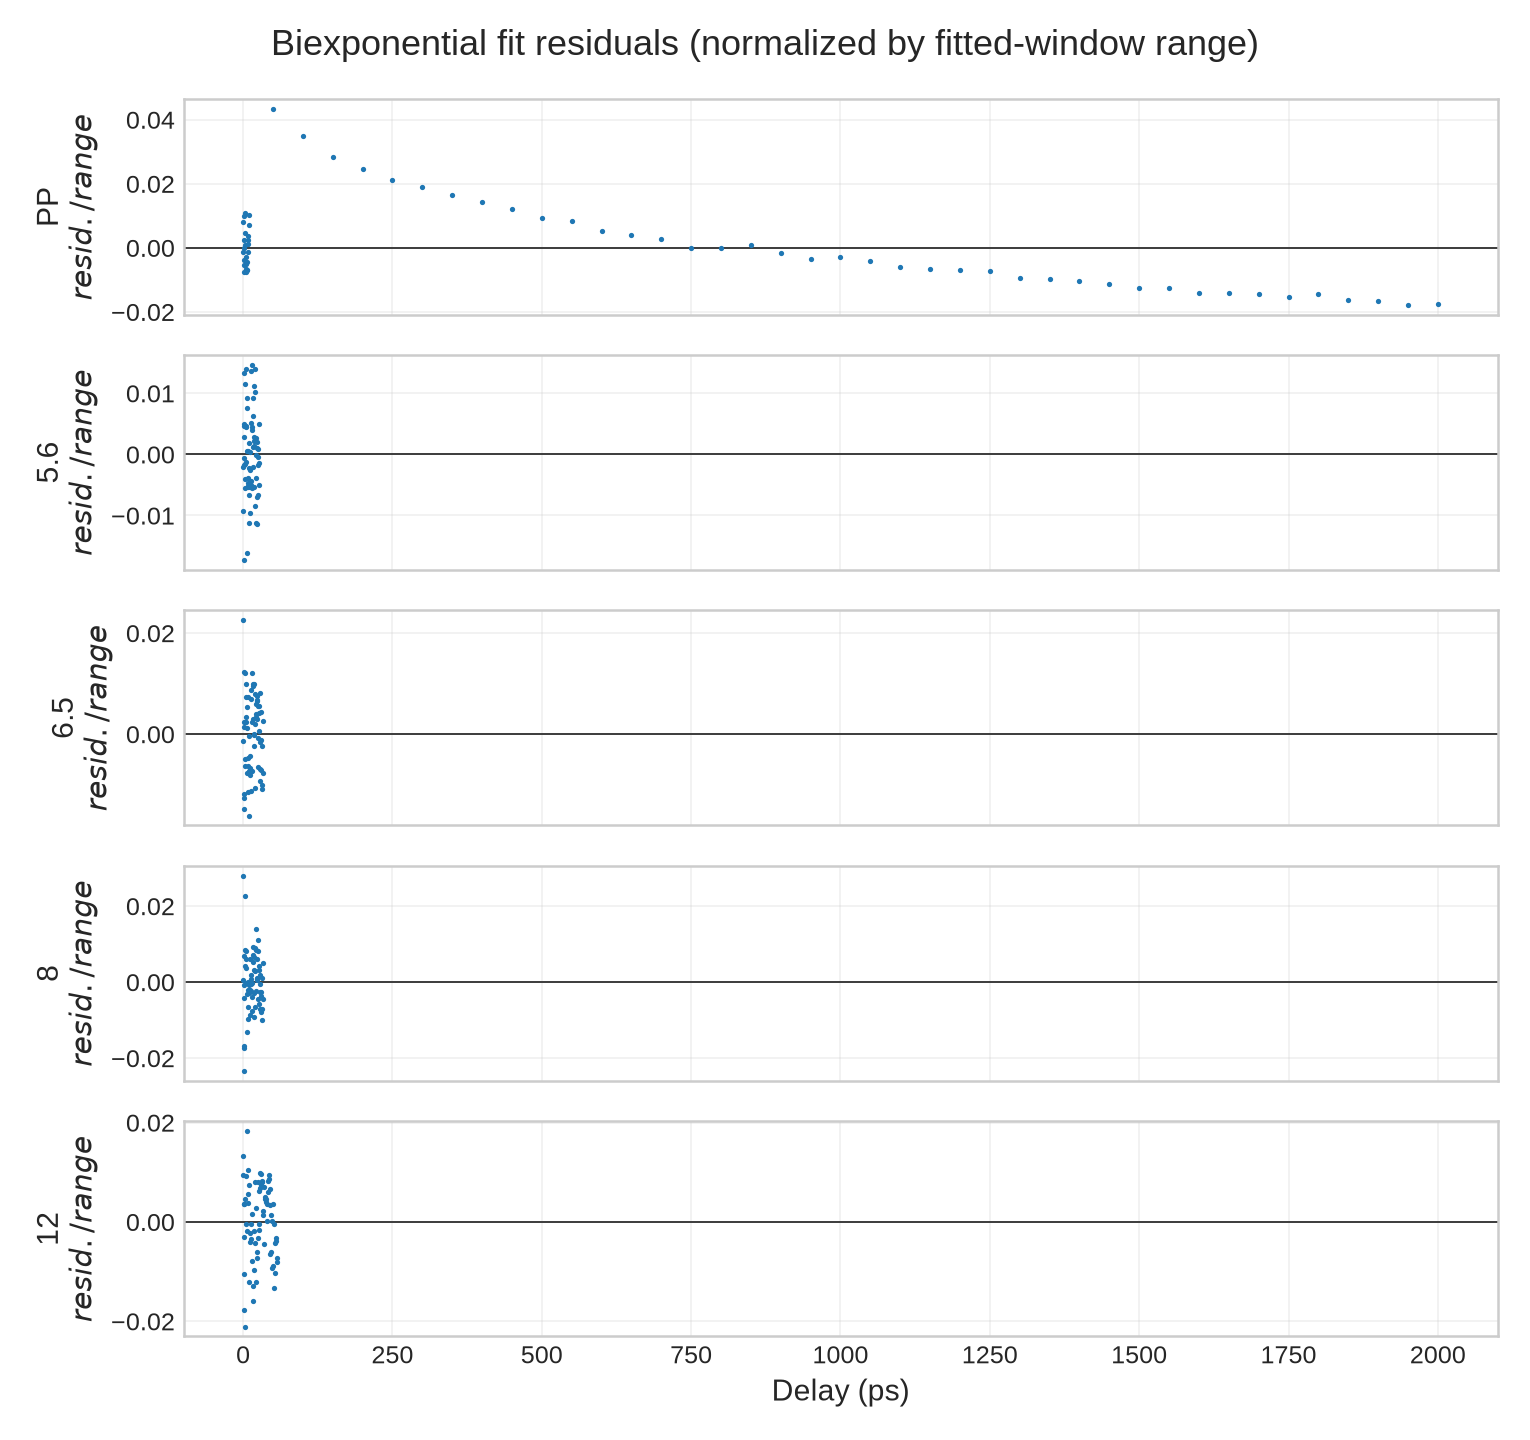
\includegraphics[width=.98\linewidth]{../plots/gaas_fit_residuals.png}
\caption{Biexponential fit residuals for the averaged data, normalized by the fitted-window signal range. The traces are displayed separately to make structure visible.}
\label{fig:fit-residuals}
\end{figure}
\begin{figure}[htbp]
\centering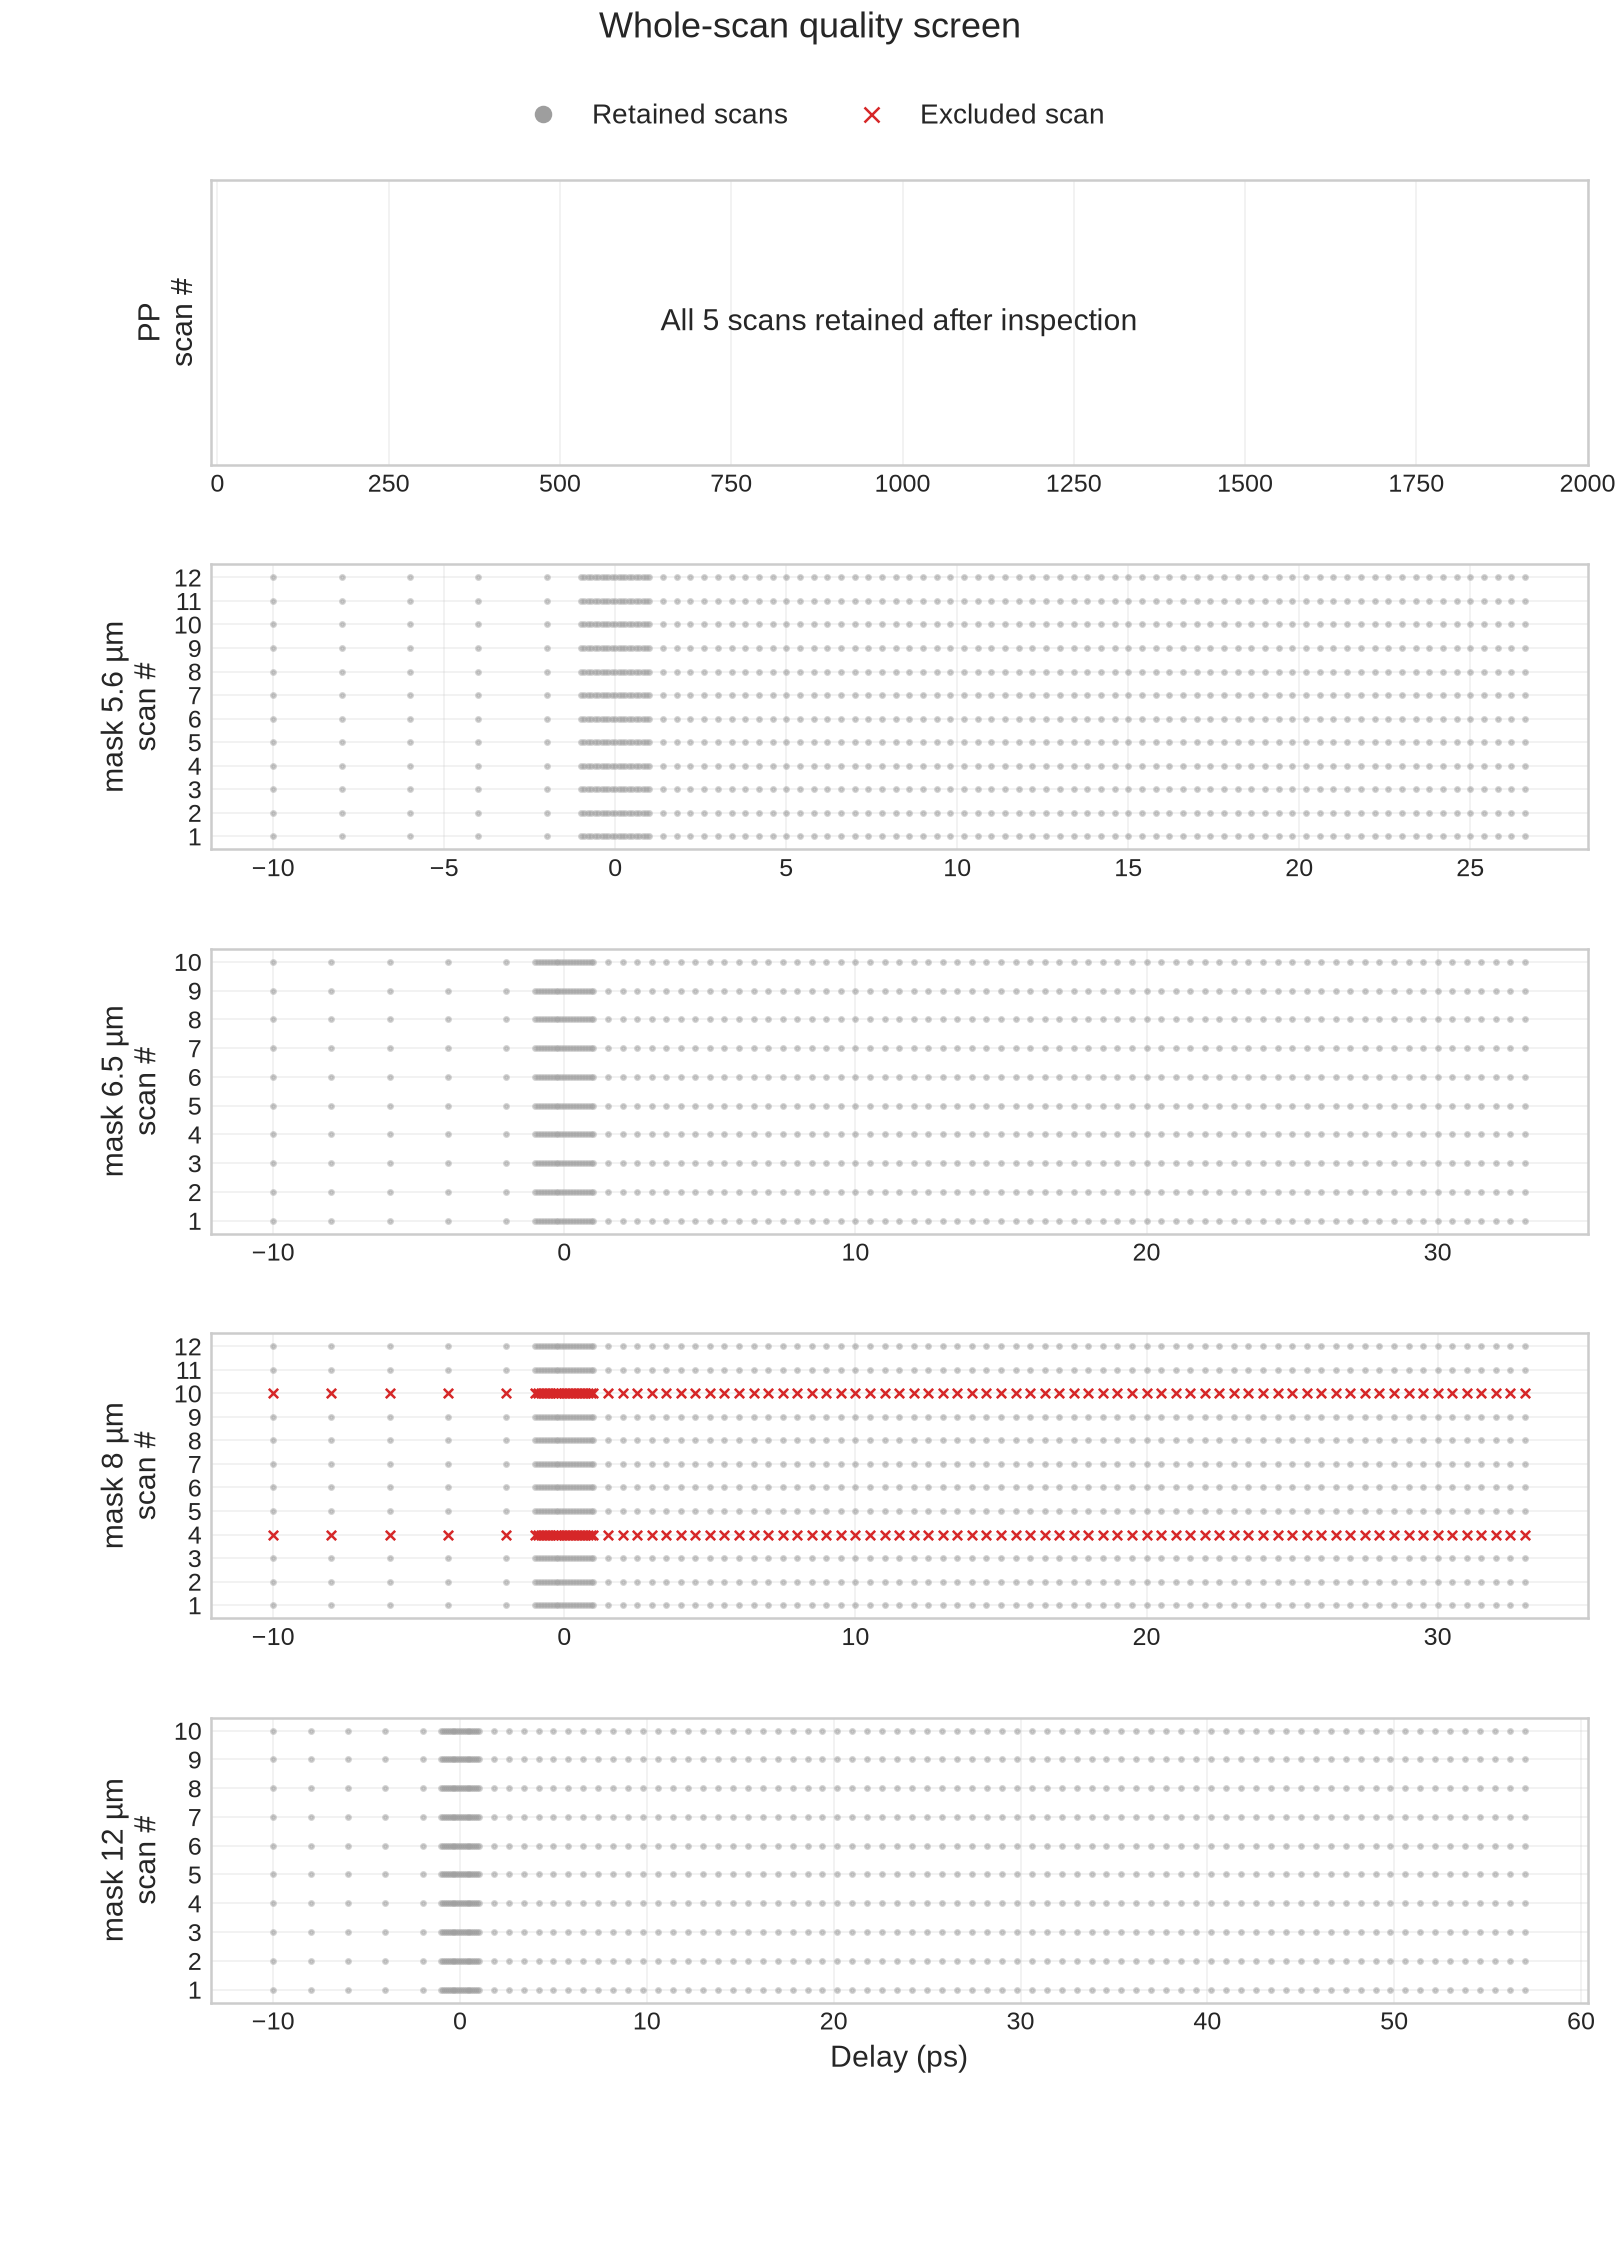
\includegraphics[width=.98\linewidth]{../plots/outlier_diagnostics.png}
\caption{Whole-scan quality screen. Red crosses mark scans excluded by the robust scan-deviation criterion; all five pump--probe scans were retained after inspection.}\label{fig:outlier-diagnostics}
\end{figure}
\begin{figure}[htbp]
\centering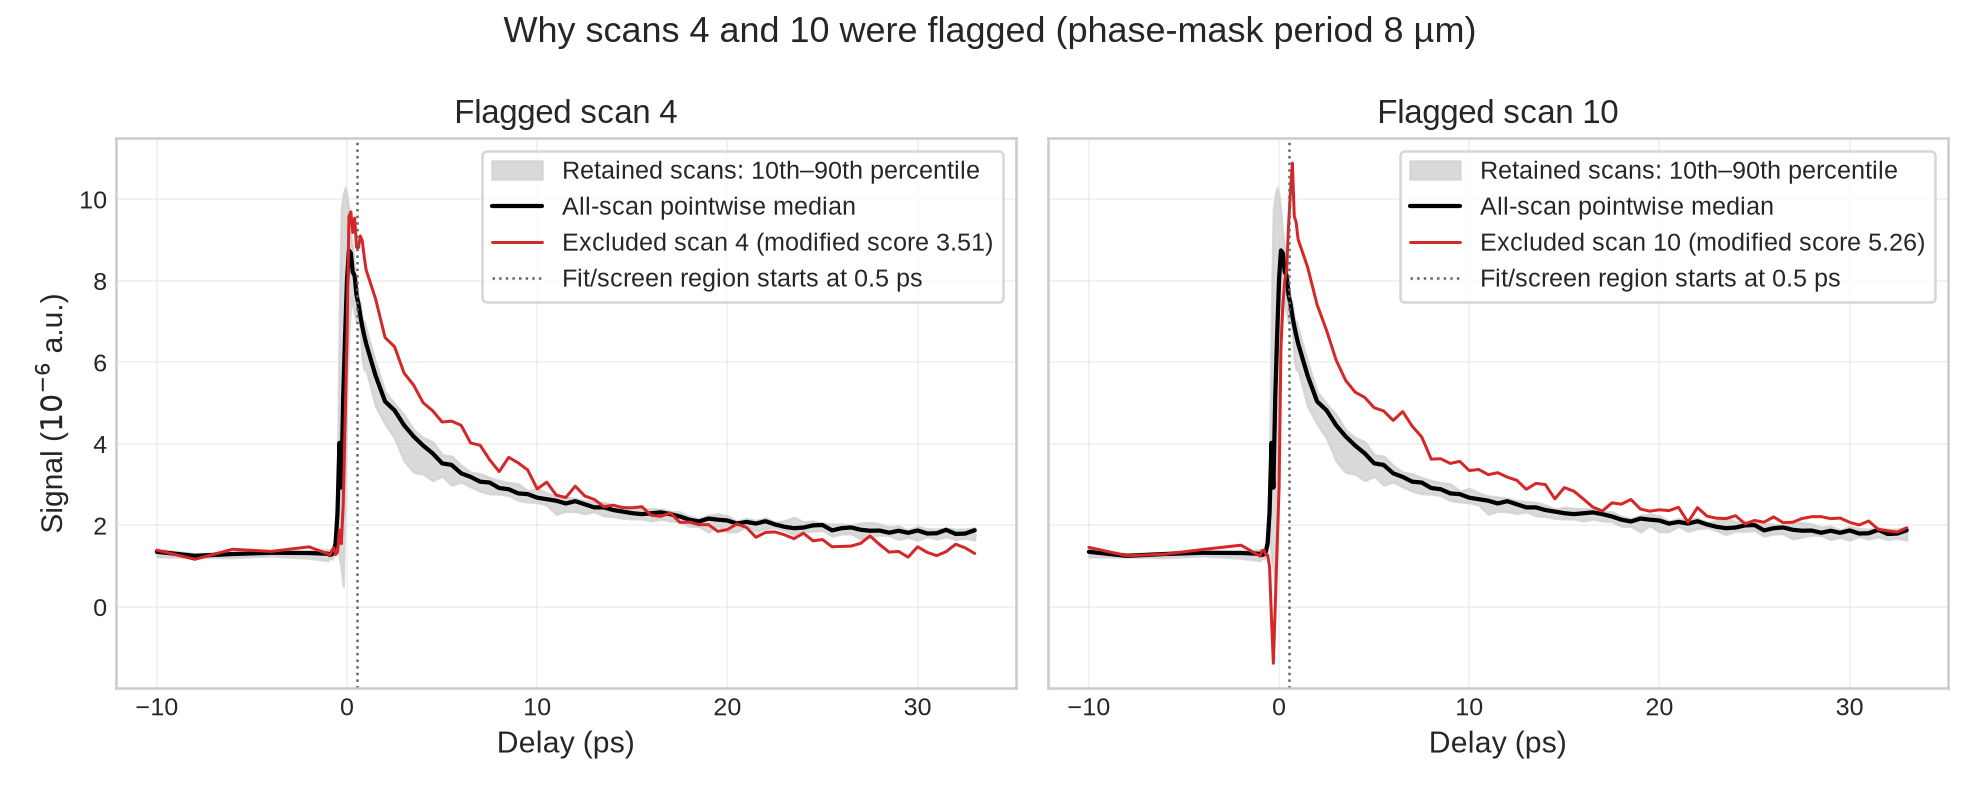
\includegraphics[width=.98\linewidth]{../plots/excluded_scan_comparison.png}
\caption{The two statistically flagged scans from the phase-mask-period-8 file, compared with the all-scan pointwise median and the 10th--90th percentile band of retained scans. The vertical dotted line marks the 0.5 ps fit/screen threshold. Scan 4 is borderline; scan 10 shows the larger deviation.}\label{fig:excluded-scan-comparison}
\end{figure}
\FloatBarrier


Table~\ref{tab:tgfits} gives the fitted fast and slow decay times. The data columns are averaged only after the scan screen; the table gives 95\% bootstrap intervals from resampling retained scans, conditional on the selected traces and model. The sample periods use the supplied quarter-period correction, and the first column of each transient file is interpreted in ps.
\begin{table}[ht]
\centering
\caption{Biexponential fit lifetimes and 95\% repeat-scan bootstrap intervals. The filename value is the phase-mask period; the sample period is one quarter of that value.}
\label{tab:tgfits}
\small
\begin{tabular}{lrrrr}\toprule
Data & $\Lambda_{\rm sample}$ (\si{\micro\metre}) & $q$ ($10^6$\,\si{\per\metre}) & $\tau_f$ (ps) & $\tau_s$ (ps)\\\midrule
Pump--probe & -- & 0 & 0.717 [0.698, 0.743] & 7.878 [7.753, 8.040]\\
TG 5.6 & 1.400 & 4.488 & 1.206 [1.031, 1.445] & 7.205 [6.412, 8.771]\\
TG 6.5 & 1.625 & 3.867 & 1.298 [1.157, 1.503] & 9.200 [8.156, 10.960]\\
TG 8 & 2.000 & 3.142 & 1.363 [1.064, 1.983] & 9.496 [7.933, 12.250]\\
TG 12 & 3.000 & 2.094 & 2.060 [1.708, 2.463] & 13.283 [11.970, 15.170]\\\bottomrule
\end{tabular}
\end{table}

\subsection{Part IV: Recombination, ambipolar diffusivity, and mobility}
For the finite-$q$ TG measurements, the slow-component rates are regressed against $q^2$ as motivated by the diffusion equation. The slope is $3.71\times10^{-15}\,\si{\metre\squared\per\pico\second}$ ($R^2=0.934$), giving a TG-only ambipolar diffusion estimate $D_a=(3.71\pm0.70)\times10^{-3}\,\si{\metre\squared\per\second}$, where the stated error is the standard error of the four-point regression slope. Resampling complete retained scans gives a 95\% bootstrap interval $[2.31,4.96]\times10^{-3}\,\si{\metre\squared\per\second}$. This interval includes repeat-scan variation but not calibration or model uncertainty. Retaining borderline scan 4 while still excluding scan 10 changes the estimate by about 2\% to $3.78\times10^{-3}\,\si{\metre\squared\per\second}$ (Fig.~\ref{fig:rate-q2}).

\begin{figure}[htbp]
\centering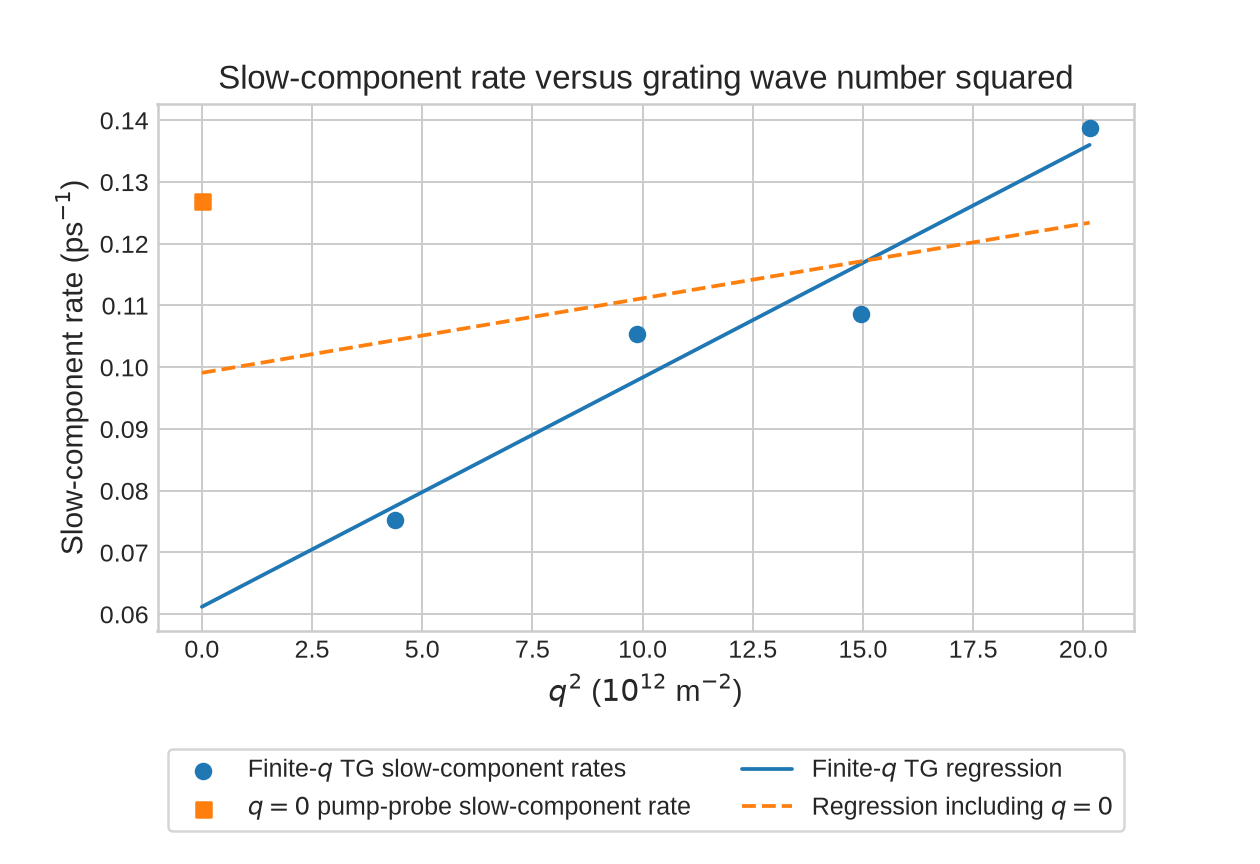
\includegraphics[width=.98\linewidth]{../plots/rate_vs_q2.png}
\caption{Slow-component rates against $q^2$ computed from the sample grating periods (one quarter of the phase-mask values). The finite-$q$ line gives the TG-only diffusion estimate; including the q=0 pump--probe rate gives a poor linear fit.}\label{fig:rate-q2}
\end{figure}

\section{Discussion}
The pulse-characterization results are internally consistent at the level of scale: the selected pulse durations are close to the \SI{83.8}{fs} Gaussian transform-limit estimate from the measured spectrum. Both fitted durations are slightly shorter than that limit. Since the formal fit errors omit delay-axis calibration, model mismatch and candidate-selection uncertainty, the small difference should not be interpreted as a statistically established violation of the transform limit.

The reflectivity traces support effective fast and slow decay constants within the fitted interval, but the biexponential form is phenomenological. It does not uniquely map either fitted lifetime to a microscopic carrier process. In particular, the experiment did not measure carrier temperature or energy distribution. The fit begins at \SI{0.5}{ps}, too late to resolve the sub-picosecond thermalization and scattering processes relevant to hot-carrier cooling. The literature times cited in Part II describe such microscopic processes under particular excitation conditions and are not direct benchmarks for our fitted reflectivity lifetimes.

The main transport result is the finite-$q$ TG slope shown in Fig.~\ref{fig:rate-q2}. The fit yields
\begin{equation*}
D_a=(3.71\pm0.70)\times10^{-3}\,\si{\metre\squared\per\second}
\quad (\text{about }37\,\si{\centi\metre\squared\per\second}).
\end{equation*}
The repeat-scan bootstrap interval is $[2.31,4.96]\times10^{-3}\,\si{\metre\squared\per\second}$. A bulk-GaAs pump--probe study reports an ambipolar diffusivity near $20\,\si{\centi\metre\squared\per\second}$ at room temperature, so the present estimate is of the same order but roughly 1.9 times larger \cite{ruzicka}. This is not a controlled like-for-like comparison because our carrier density, fluence and sample temperature are unavailable; density-dependent effects can also change GaAs diffusivity \cite{young}.

The finite-$q$ regression intercept corresponds to a nominal recombination time of \SI{16.3}{ps}. The pump--probe slow rate instead corresponds to \SI{7.878}{ps}, about twice the TG extrapolation; including the $q=0$ point reduces the linear-fit $R^2$ to 0.161. This disagreement is the central limitation of the pump--probe comparison: the $q=0$ reflectivity signal and finite-$q$ diffracted signal may weight different relaxation channels, while the simple rate law assumes one common population and one recombination intercept. Thus the TG-only slope is an exploratory estimate, and the intercept should not be reported as a measured recombination lifetime.

Using $\mu_a=eD_a/(k_BT)$ at an assumed $T=\SI{300}{K}$ gives a conditional mobility of about $1.44\times10^3\,\si{\centi\metre\squared\per\volt\per\second}$. The sample temperature was not logged, and the Einstein conversion assumes non-degenerate carriers in thermal equilibrium at a common temperature. Therefore this mobility is conditional on assumptions rather than a direct measurement. Across the analysis, the main unresolved uncertainties are the delay and grating-period calibrations, the fit interval and biexponential model, limited grating-period sampling, scan-selection sensitivity, and missing acquisition metadata.

\section{Conclusion}
The supplied measurements support pulse-duration estimates near \SI{80}{fs} and effective fast and slow transient-decay times. The spectral transform-limit comparison is close, although systematic uncertainties are larger than the formal fit errors. The data do not directly determine hot-carrier cooling or an electron--phonon coupling coefficient. The finite-$q$ TG rates produce an exploratory ambipolar-diffusivity estimate of $(3.71\pm0.70)\times10^{-3}\,\si{\metre\squared\per\second}$ and a conditional mobility estimate if room temperature is assumed. The mismatch between the pump--probe rate and TG extrapolation, together with sparse wave-number sampling and missing experimental metadata, prevents a firm recombination-lifetime determination or a strong literature comparison.

\begin{thebibliography}{9}
\bibitem{tutorial} Institute of Physics II, University of Cologne, \emph{M2.10: Ultrafast Transient Grating Spectroscopy}, practical-course tutorial, version December 2019, especially Eqs.~(4.2)--(4.14) and Secs.~5--6.
\bibitem{hunsche} S. Hunsche, H. Heesel, A. Ewertz, H. Kurz, and J. H. Collet, ``Spectral-hole burning and carrier thermalization in GaAs at room temperature,'' \emph{Physical Review B} \textbf{48}, 17818 (1993), doi:10.1103/PhysRevB.48.17818.
\bibitem{ruzicka} B. A. Ruzicka, L. K. Werake, H. Samassekou, and H. Zhao, ``Ambipolar diffusion of photo-excited carriers in bulk GaAs,'' \emph{Applied Physics Letters} \textbf{97}, 262119 (2010), doi:10.1063/1.3533664.
\bibitem{kash} J. A. Kash, J. C. Tsang, and J. M. Hvam, ``Subpicosecond Time-Resolved Raman Spectroscopy of LO Phonons in GaAs,'' \emph{Physical Review Letters} \textbf{54}, 2151 (1985), doi:10.1103/PhysRevLett.54.2151.
\bibitem{leheny} R. F. Leheny, J. Shah, R. L. Fork, C. V. Shank, and A. Migus, ``Dynamics of hot carrier cooling in photo-excited GaAs,'' \emph{Solid State Communications} \textbf{31}, 809--813 (1979), doi:10.1016/0038-1098(79)90393-4.
\bibitem{young} J. F. Young and H. M. van Driel, ``Ambipolar diffusion of high-density electrons and holes in Ge, Si, and GaAs: Many-body effects,'' \emph{Physical Review B} \textbf{26}, 2147 (1982), doi:10.1103/PhysRevB.26.2147.
\end{thebibliography}

\section*{AI Use Disclosure}
\addcontentsline{toc}{section}{AI Use Disclosure}
Generative AI was used to assist with data-analysis code, plotting, and editing the presentation of this report. The authors reviewed the analysis, calculations, figures, and final text and remain responsible for their accuracy and conclusions.
\end{document}
